Time series are generated and stored at a vastly increasing rate in many industrial and research applications, including the Web and the Internet of Things, public utilities, finance, astronomy, biology, and many more. A significant portion concerns \emph{geolocated} time series, i.e., those generated at, or otherwise associated with specific locations. While indexing, mining and exploring time series data has attracted a lot of interest from the database and data mining communities \cite{camerra2014kais,ding2008pvldb,shieh2008kdd,paraskevopoulos2017icdm}, studying of geolocated time series is still largely overlooked.

Geolocated time series can be found in various domains and applications. A typical example is encountered in the \textit{DAIAD} project\footnote{\url{http://daiad.eu/}}, where time series are used to represent water consumption measured by smart meters installed in urban households. Analyzing such time series can provide valuable insights regarding trends and patterns of consumer behavior in daily life. Such results can then be used to forecast and balance water demand, as well as to plan and prioritize interventions that can guide consumers towards more sensible water use. Similar use cases can also be found in other domains, such as in geomarketing or mobile advertisement, where geolocated time series may represent the number of visitors or the revenue generated at a certain location across time. Extracting insights, trends and patterns can be significantly facilitated by {\em map-based visualizations} of {\em summarized} time series data. For example, such visualizations can reveal which type of consumption patterns are most frequently observed among consumers in a certain area or what the spatial distribution of sales for a certain product looks like. 

\begin{comment}
In all these cases, visually exploring such time series in conjunction with the locations where these are generated, can enable extraction of useful insights regarding behavioral patterns and their geographic distribution, as well as the discovery of trends or anomalies that could indicate interesting events for further examination.
\end{comment}

However, time series is an inherently complex data type, and such datasets can reach extremely large volumes, both horizontally (i.e., very long series across time) and vertically (i.e., time series generated by countless sources). Consequently, management, analysis and exploration of such Big Time Series Data is a task of excessive complexity, requiring efficient algorithms. In particular, visual exploration of geolocated time series needs to process the required information in real time, while the user interacts with the map. Whenever the user zooms in or scrolls the map, visual analytics and aggregates should be computed on-the-fly, e.g., identifying the predominant patterns in the time series and their spatial distribution within the map area.

Consider the example illustrated in Figure~\ref{fig:map}. When the user zooms the map into the red rectangle, the visualization tool should readily identify and present the two patterns (shown in blue and green color) appearing therein. To avoid cluttering the map, when the spatial distribution is very dense or the map area is too large, it is meaningful to display only aggregate information, e.g., the number of time series per identified pattern and their respective centroids; individual time series may be identified only at a greater zoom level.

Such fast computation and retrieval for large datasets of geolocated time series can be enabled by indexing. Several approaches have been proposed that efficiently index large amounts of plain time series data, either relying on \emph{Discrete Wavelet Transform} like \cite{chan1999icde} to reduce dimensionality of time series, or the family of indices based on \emph{Symbolic Aggregate Approximation} (SAX) over the time series \cite{shieh2008kdd,camerra2010icdm,camerra2014kais,zoumpatianos2014sigmod}. However, all aforementioned techniques index the data solely on the time series domain, not taking the spatial dimension into account. If the analyzed time series are inherently associated with a spatial attribute (e.g., locations of smart meters), such indexing does not efficiently support queries and visualizations that do not simply apply to the time series domain, but also involve spatial filters. As in the example of Figure~\ref{fig:map}, a user may need to explore time series similar to a specific pattern, but also having locations within the actual map area. For such mixed requests, it is inefficient to evaluate each predicate separately, e.g., using first the time series index to retrieve a candidate set of time series similar to the pattern, and then applying a spatial filter against these candidates to retrieve only those qualifying within the specified query area. 

\begin{figure}[t]
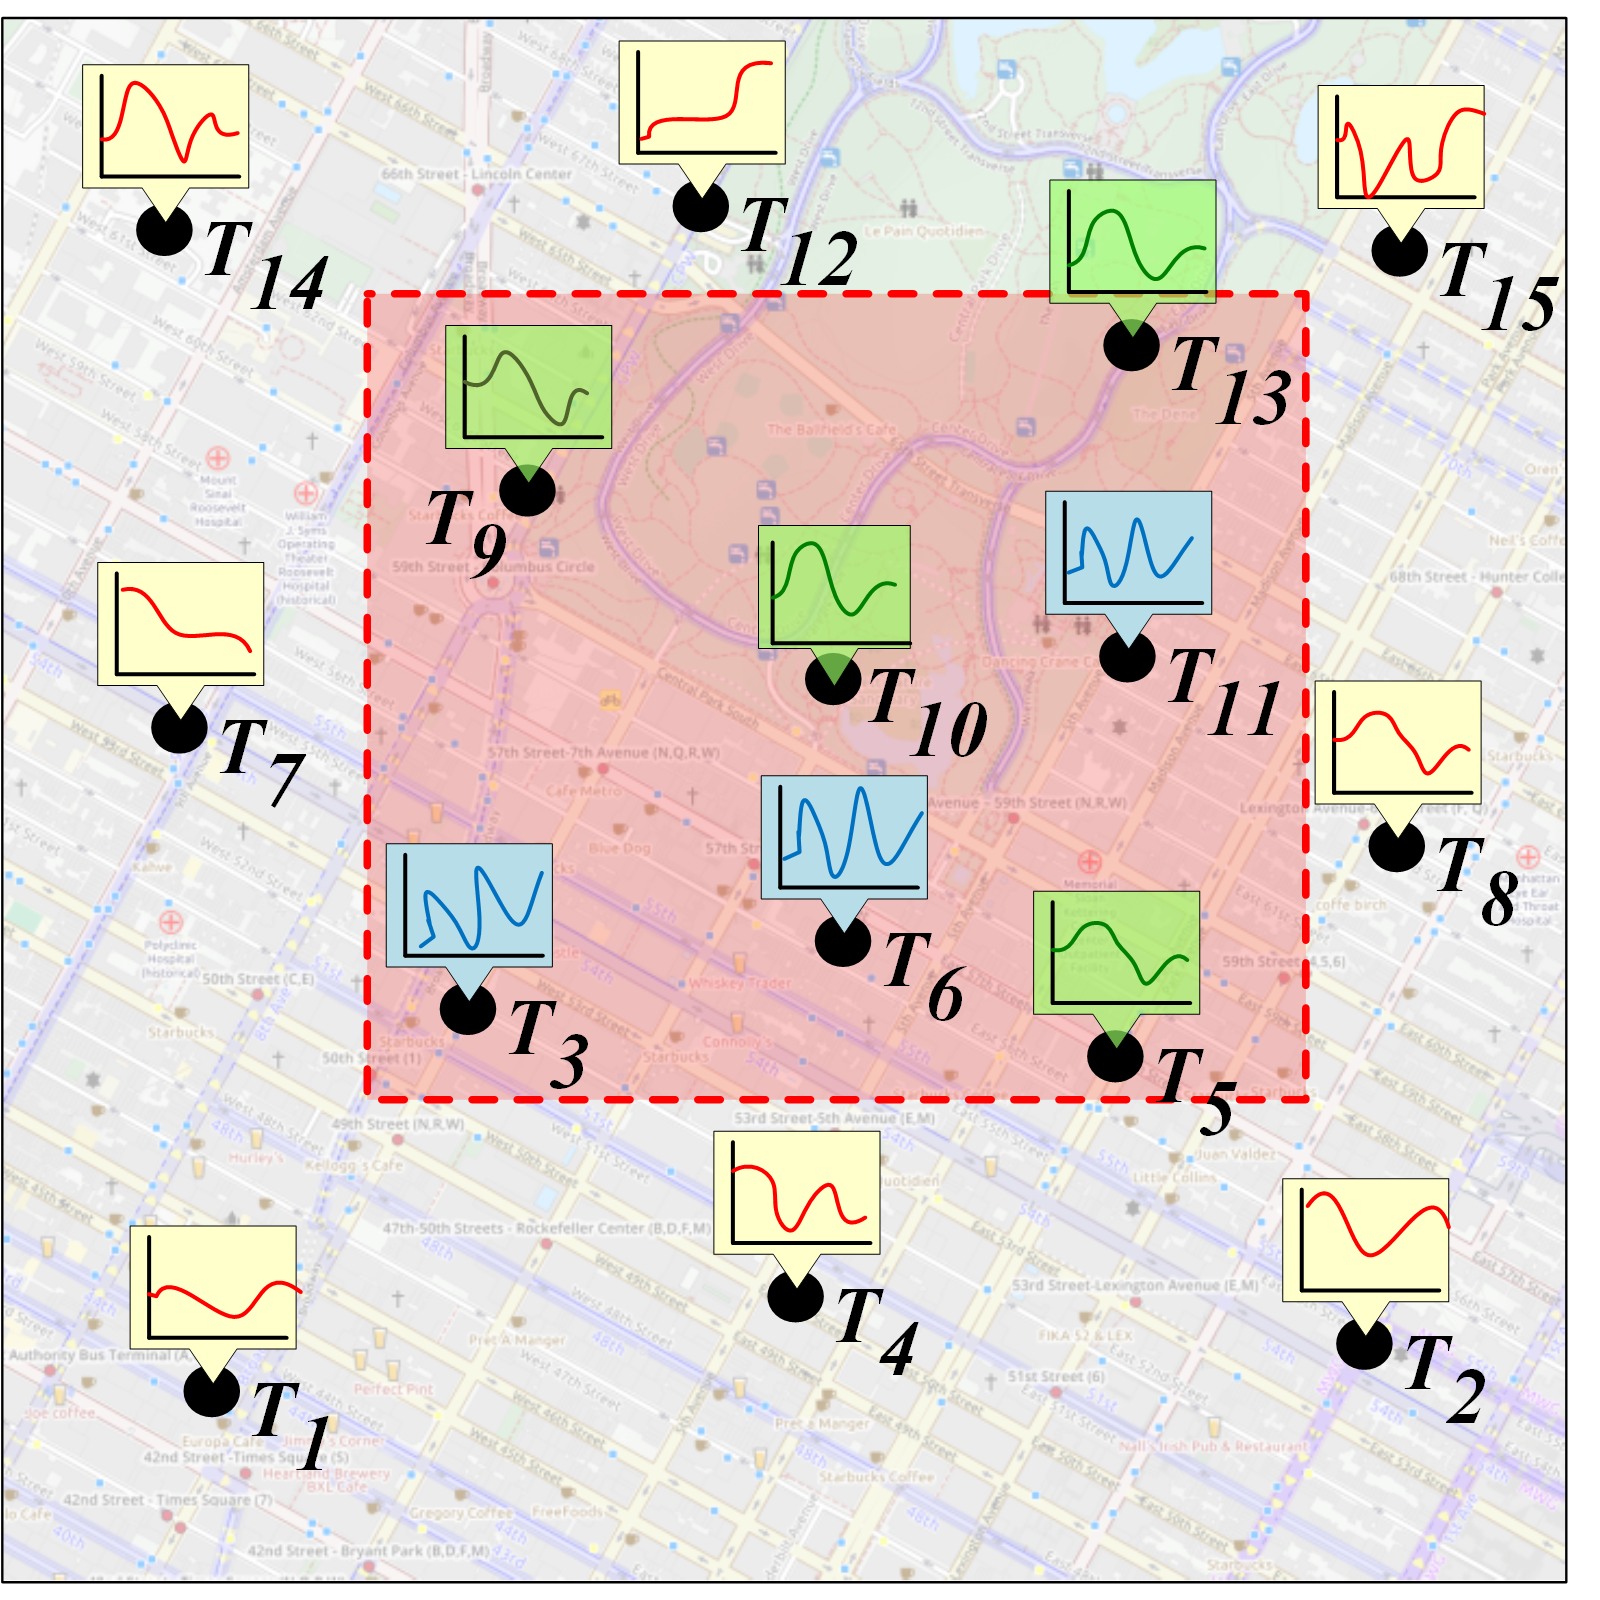
\includegraphics[width=0.32\textwidth]{figures/map.png}
\vspace{-5pt}
\caption{Exploring time series patterns in a spatial region.}
\vspace{-15pt}
\label{fig:map}
\end{figure}

To address this shortcoming, we have recently proposed an extension to the R-tree spatial index \cite{Guttman1984}, offering efficient support to similarity search on geolocated time series. The idea behind our \emph{\btsr} hybrid index \cite{chatzig17btsr} is to combine both spatial proximity and time series similarity. To that end, in addition to the standard \emph{Minimum Bounding Rectangle} (MBR) denoting the spatial bound of its contents, each node is augmented with a \emph{Minimum Bounding Time Series} (MBTS), i.e., a band with upper and lower bounds that encloses all time series contained in its subtree. Maintaining both kinds of bounds per node enables pruning the search space simultaneously in the spatial and the time series domains while traversing the index. To increase pruning effectiveness, time series indexed in a given node are further distinguished into {\em bundles} on the basis of their similarity, hence achieving tighter bounds in the MBTS of these bundles.


%%%%%%%%%%%%%%%%%%%%%%%%%%%%%%%%%%%%%%%%%
\begin{comment}

Thus, the number of required node accesses is significantly reduced, since we only retrieve the contents of nodes that may actually contain objects satisfying both types of predicates.
\end{comment}

\begin{comment}
\snote{[Could be removed: } Various approaches have introduced visualization techniques that allow for the efficient exploration of time series data, as well as data of spatio-temporal nature. Time series summarization techniques can facilitate the extraction of possible patterns within time series collections. \snote{...more regarding existing time series and spatio-temporal visualizations could go here....}. However, to the best of our knowledge, none of the existing works so far has considered the specific case of geolocated time series. \snote{]}
\end{comment}
%%%%%%%%%%%%%%%%%%%%%%%%%%%%%%%%%%%%%%%%%

In this paper, we take advantage of this novel \btsr index and propose an interactive method for map-based visual exploration and summarization over large datasets of geolocated time series. Intuitively, when the user interacts with the map, i.e., either zooms in/out or moves the visible area, this technique can identify the most significant patterns characterizing the time series located in this area. These patterns are abstracted by the MBTSs of the bundles contained in the nodes of the \btsr index within this area, summarizing the various time series therein. In addition, the corresponding MBRs and the number of geolocated time series per pattern can be depicted on the map. 

For providing prompt visualizations of summaries over geolocated time series data and minimizing latency when drawing the relevant graphic elements, we need early access to both spatial and time series information while traversing the index. For this purpose, we adapt the \btsr index so as to also include aggregates per node, i.e., the number of time series pertaining to each bundle. Subsequently, we introduce a new traversal algorithm for efficient retrieval of a given number of bundles that are the most representative in the map area. To the best of our knowledge, this is the first work that considers visual exploration and summarization of geolocated time series.

%%%%%%%%%%%%%%%%%%%%%%%%%%%%%%%%%%%%%%
\begin{comment}
This technique  which allows interactive, real-time extraction and visualization of aggregate time series along with their corresponding containing areas on a map, using an adapted version of the \btsr index. 
\end{comment}
%%%%%%%%%%%%%%%%%%%%%%%%%%%%%%%%%%%%%%



In summary, our main contributions are as follows:

\begin{itemize}
 \item We propose an adapted variant of the \btsr index as well as a novel algorithm for its traversal in order to quickly retrieve summaries (bundles) of geolocated time series within a given area.
 \item Thanks to robust index support, we introduce a method that can cluster bundles according to time series similarity, calculate their support and identify their spatial extent, thus enabling their interactive map-based exploration.
 \item We exemplify the proposed visualization method with two use cases based on real-world datasets.
 \item We also empirically evaluate the performance of index traversal, confirming its low execution cost against a large synthetic dataset of geolocated time series.
\end{itemize}



The remainder of this paper is organized as follows. Section~\ref{sec:related} reviews related work. Section~\ref{sec:problem} outlines basic concepts and formulates the problem. Section~\ref{sec:approach} describes the \btsr index and introduces our approach on summarization of geolocated time series for their efficient visual exploration. Section~\ref{sec:evaluation} presents indicative use cases with map visualizations and also reports performance results. Finally, Section~\ref{sec:conclusions} concludes the paper and outline future research directions.

